线性表是具有相同特性数据元素的一个有限序列。该序列中所含元素的个数叫做线性表的长度,用n(n≥0)表示。

{\textbf{1. 顺序表的结构定义}}{}

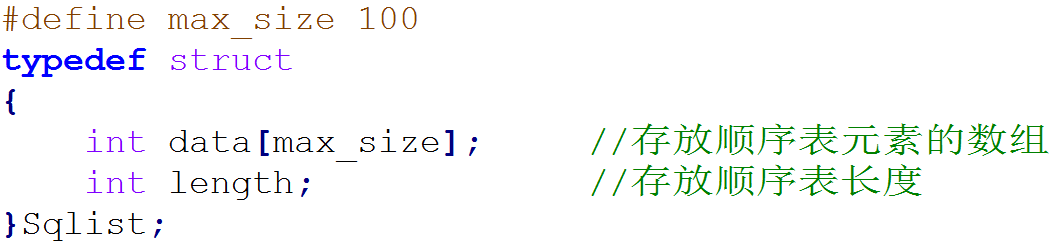
\includegraphics[width=3.33333in,height=0.77083in]{png-jpeg-pics/858F0B2FB24FD4CAC49A48E3B93C504F.png}

{上面是结构体定义,考试中直接定义数组即可。如下:\\
}

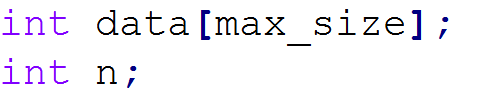
\includegraphics[width=1.25000in,height=0.22917in]{png-jpeg-pics/BB30D5618AFCED398847C5DFD44A84A8.png}

{\textbf{2. 单链表结点定义}}

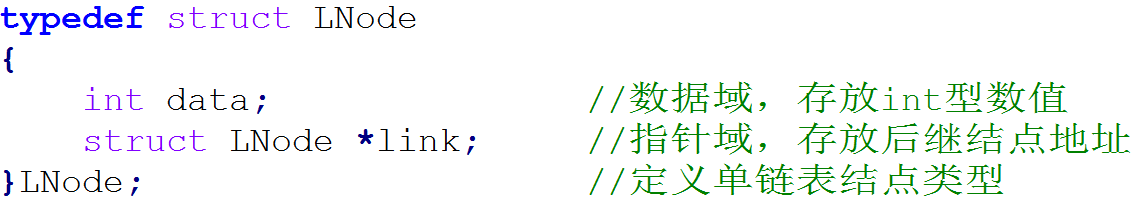
\includegraphics[width=3.33333in,height=0.58333in]{png-jpeg-pics/A6664F2AC886BAD99E87039DD7E68251.png}

{\textbf{{3. 双链表结点定义}}\\
}

{跟二叉树结点的定义很像。\\
}

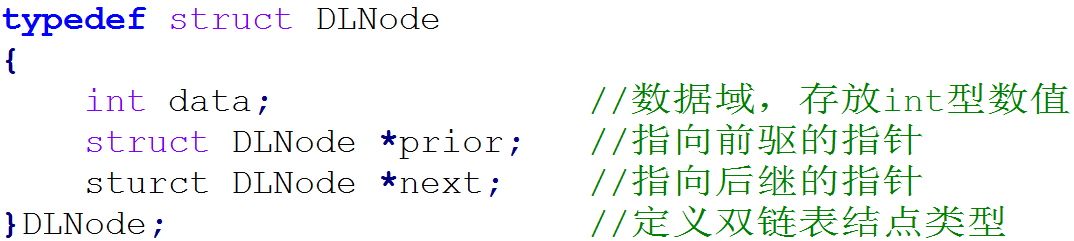
\includegraphics[width=3.33333in,height=0.75000in]{png-jpeg-pics/B2D7F23BD5AAA4BC6D2D78B5E94D4612.png}
